
%(BEGIN_QUESTION)
% Copyright 2009, Tony R. Kuphaldt, released under the Creative Commons Attribution License (v 1.0)
% This means you may do almost anything with this work of mine, so long as you give me proper credit

Read and outline the ``Flow Through a Venturi Tube'' subsection of the ``Fluid Mechanics'' section of the ``Physics'' chapter in your {\it Lessons In Industrial Instrumentation} textbook.  Note the page numbers where important illustrations, photographs, equations, tables, and other relevant details are found.  Prepare to thoughtfully discuss with your instructor and classmates the concepts and examples explored in this reading.

\underbar{file i04036}
%(END_QUESTION)





%(BEGIN_ANSWER)


%(END_ANSWER)





%(BEGIN_NOTES)

As fluid moves through a venturi tube (a tube that narrows and then expands back to its former diameter), the fluid must accelerate through the constriction.  This increases the kinetic energy of the fluid molecules as they pass through the constriction.  As kinetic energy increases, potential energy of the fluid molecules must decrease at the same time, resulting in a decrease in pressure at the venturi tube's throat.

\vskip 10pt

The fluid pressure mostly ``recovers'' as it slows back down in the tail of the venturi tube.  Some pressure is lost permenantly, due to frictional energy losses through the venturi tube, but this is usually minimal.

\vskip 10pt

If piezometer tubes and pitot tubes are installed in am ideal venturi, the pressure and velocity heads may be shown by the liquid heights inside those tubes:

$$\includegraphics[width=15.5cm]{i04036x01.eps}$$

$$z_1 + {v_1^2 \over {2 g}} + {P_1 \over \gamma} = z_2 + {v_2^2 \over {2 g}} + {P_2 \over \gamma} = z_3 + {v_3^2 \over {2 g}} + {P_3 \over \gamma}$$














\vskip 20pt \vbox{\hrule \hbox{\strut \vrule{} {\bf Suggestions for Socratic discussion} \vrule} \hrule}

\begin{itemize}
\item{} Referencing the illustration in the textbook, explain the significance of all the ``heads'' shown in red.
\item{} Describe at least one practical application of a {\it venturi tube} besides flow measurement.
\item{} Explain why fluid pressure ``recovers'' downstream of a venturi tube.
\item{} Explain why all the Pitot-tube piezometers show the same fluid height, while the static piezometers show different fluid heights.
\end{itemize}

%INDEX% Reading assignment: Lessons In Industrial Instrumentation, Fluid Mechanics (flow through a venturi tube)

%(END_NOTES)


